\begin{frame}
    \bigcenter{Why is automated testing for Scratch difficult?}
\end{frame}

\begin{frame}\frametitle{Why is automated testing for Scratch difficult?}
    Functional testing for Scratch is not a straightforward task:
    \begin{itemize}
        \item \textcolor{upfim}{no functions} that take parameters and return a value
        \item Scratch is normally only accessible through its GUI, which is not accessible in a programmable way
        \item \textcolor{upfim}{no textual IO}, keyboard and mouse input and graphical output
    \end{itemize}

    \bigskip

    \centering
    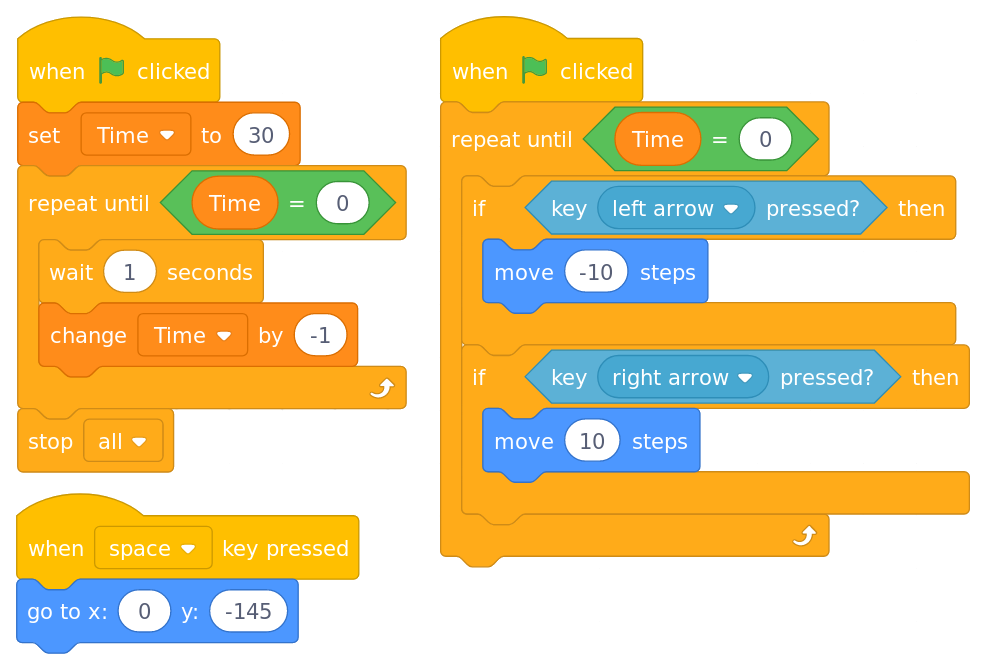
\includegraphics[width=.45\textwidth]{scratch-code}
    \hspace{1em}
    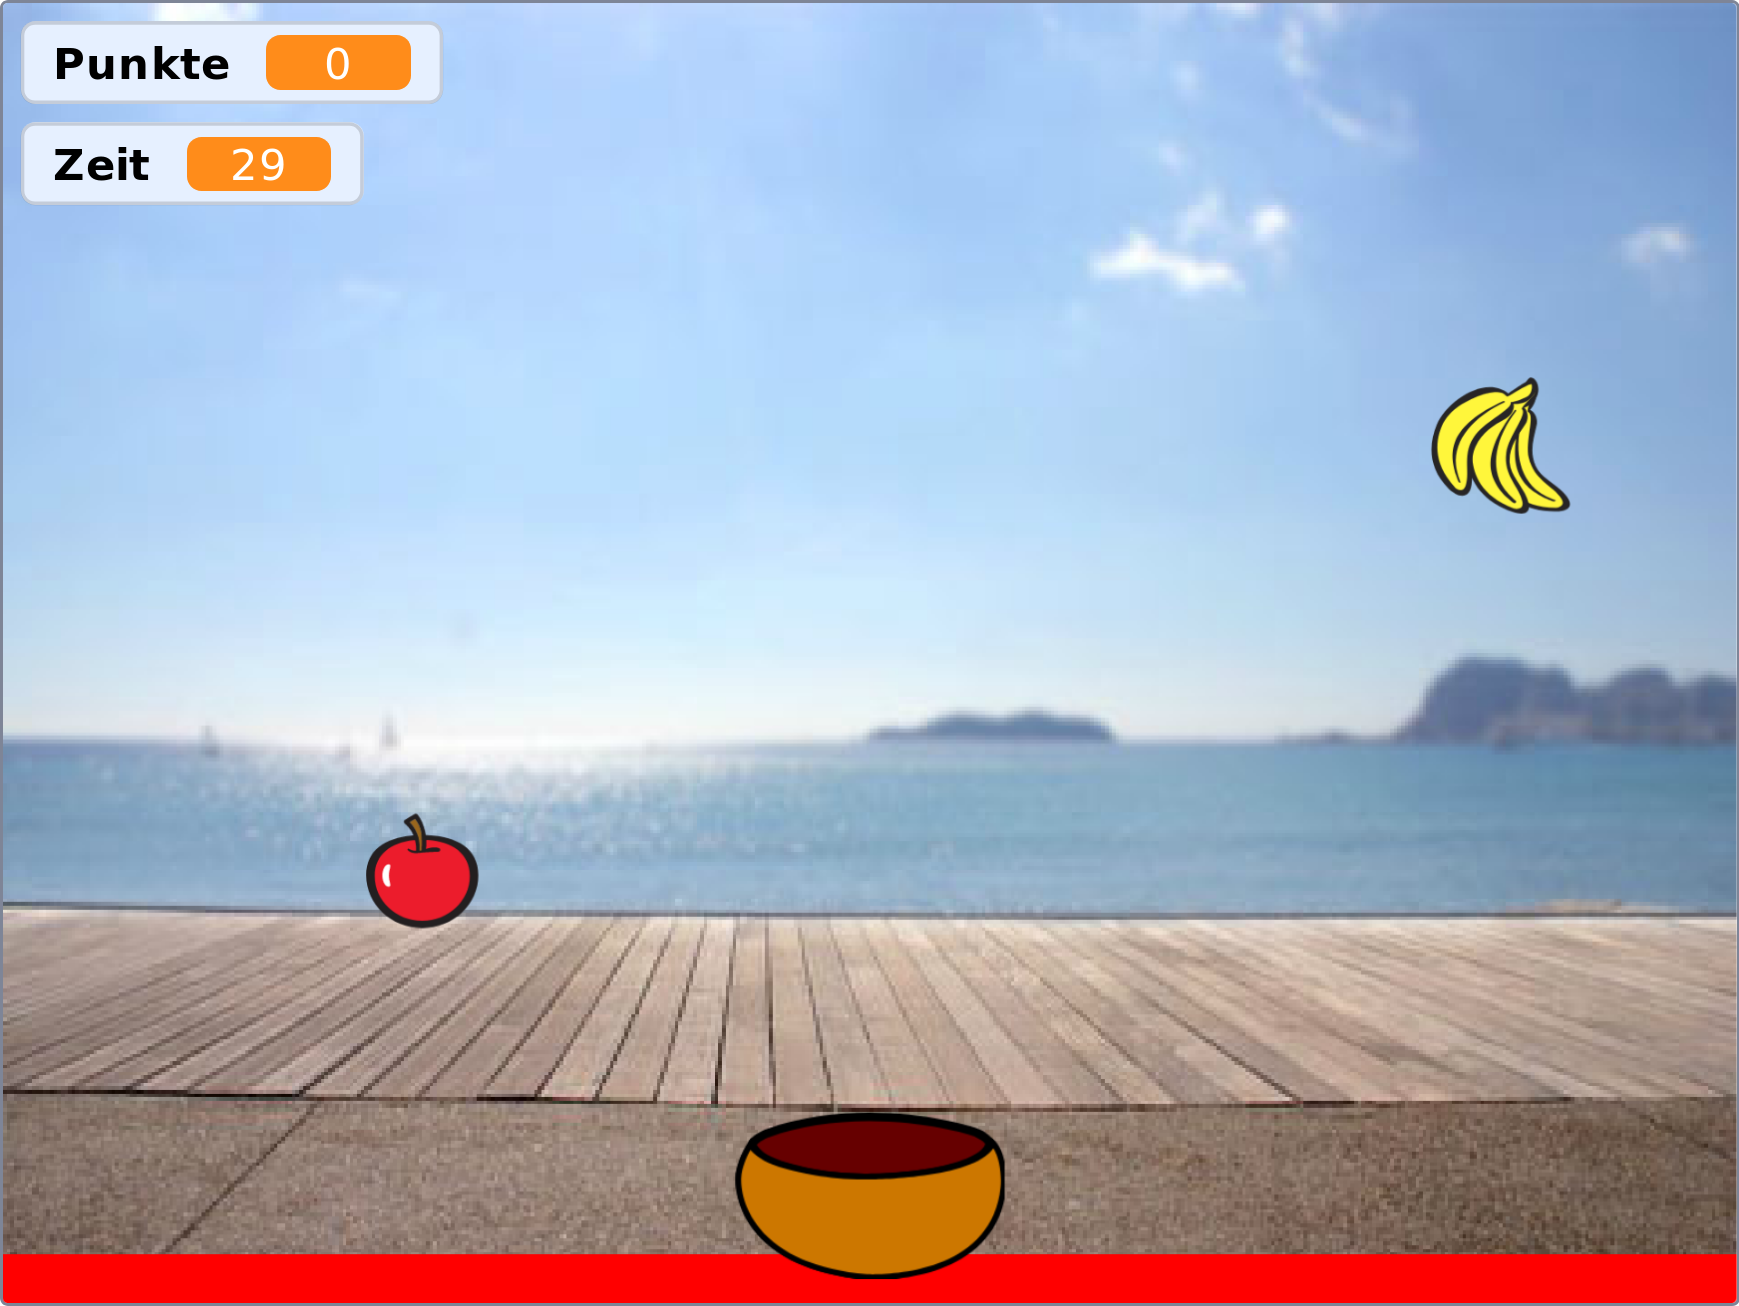
\includegraphics[width=.4\textwidth]{scratch-stage}
\end{frame}

\begin{frame}
    \bigcenter{How to test Scratch programs?}
\end{frame}

\begin{frame}[fragile]\frametitle{How to test Scratch programs? Automating IO}
    Approach: Test on a system level by automating Scratch's IO

    \begin{center}

    \tikzset{>=latex,
           arrow/.style={draw, -{Latex[length=1.5mm, width=1.5mm]}},
             put/.style={draw, minimum height=0.65cm, minimum width=1.75cm, rounded corners, fill=red!20, text width=2.4cm, text centered},
              vm/.style={draw, minimum height=1.75cm, minimum width=3.0cm, rounded corners, fill=white},
             gui/.style={draw, minimum height=2.6cm, minimum width=3.5cm, rounded corners, fill=blue!20},
         whisker/.style={draw, minimum height=2.6cm, minimum width=3.5cm, rounded corners, fill=green!20},
             box/.style={draw,text centered, rounded corners}}

    \hspace{2mm}\begin{tikzpicture}[scale=0.9, every node/.style={scale=0.9}]
        \node[box] at (0.0, 4.0) (input)  {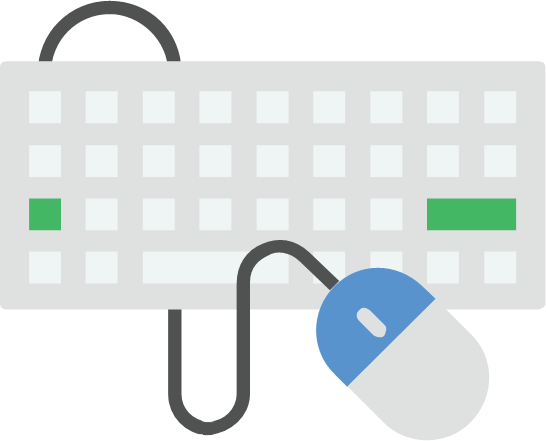
\includegraphics[height=.25\textheight]{mouse-keyboard}};
        \node[box] at (5.1, 4.0) (output) {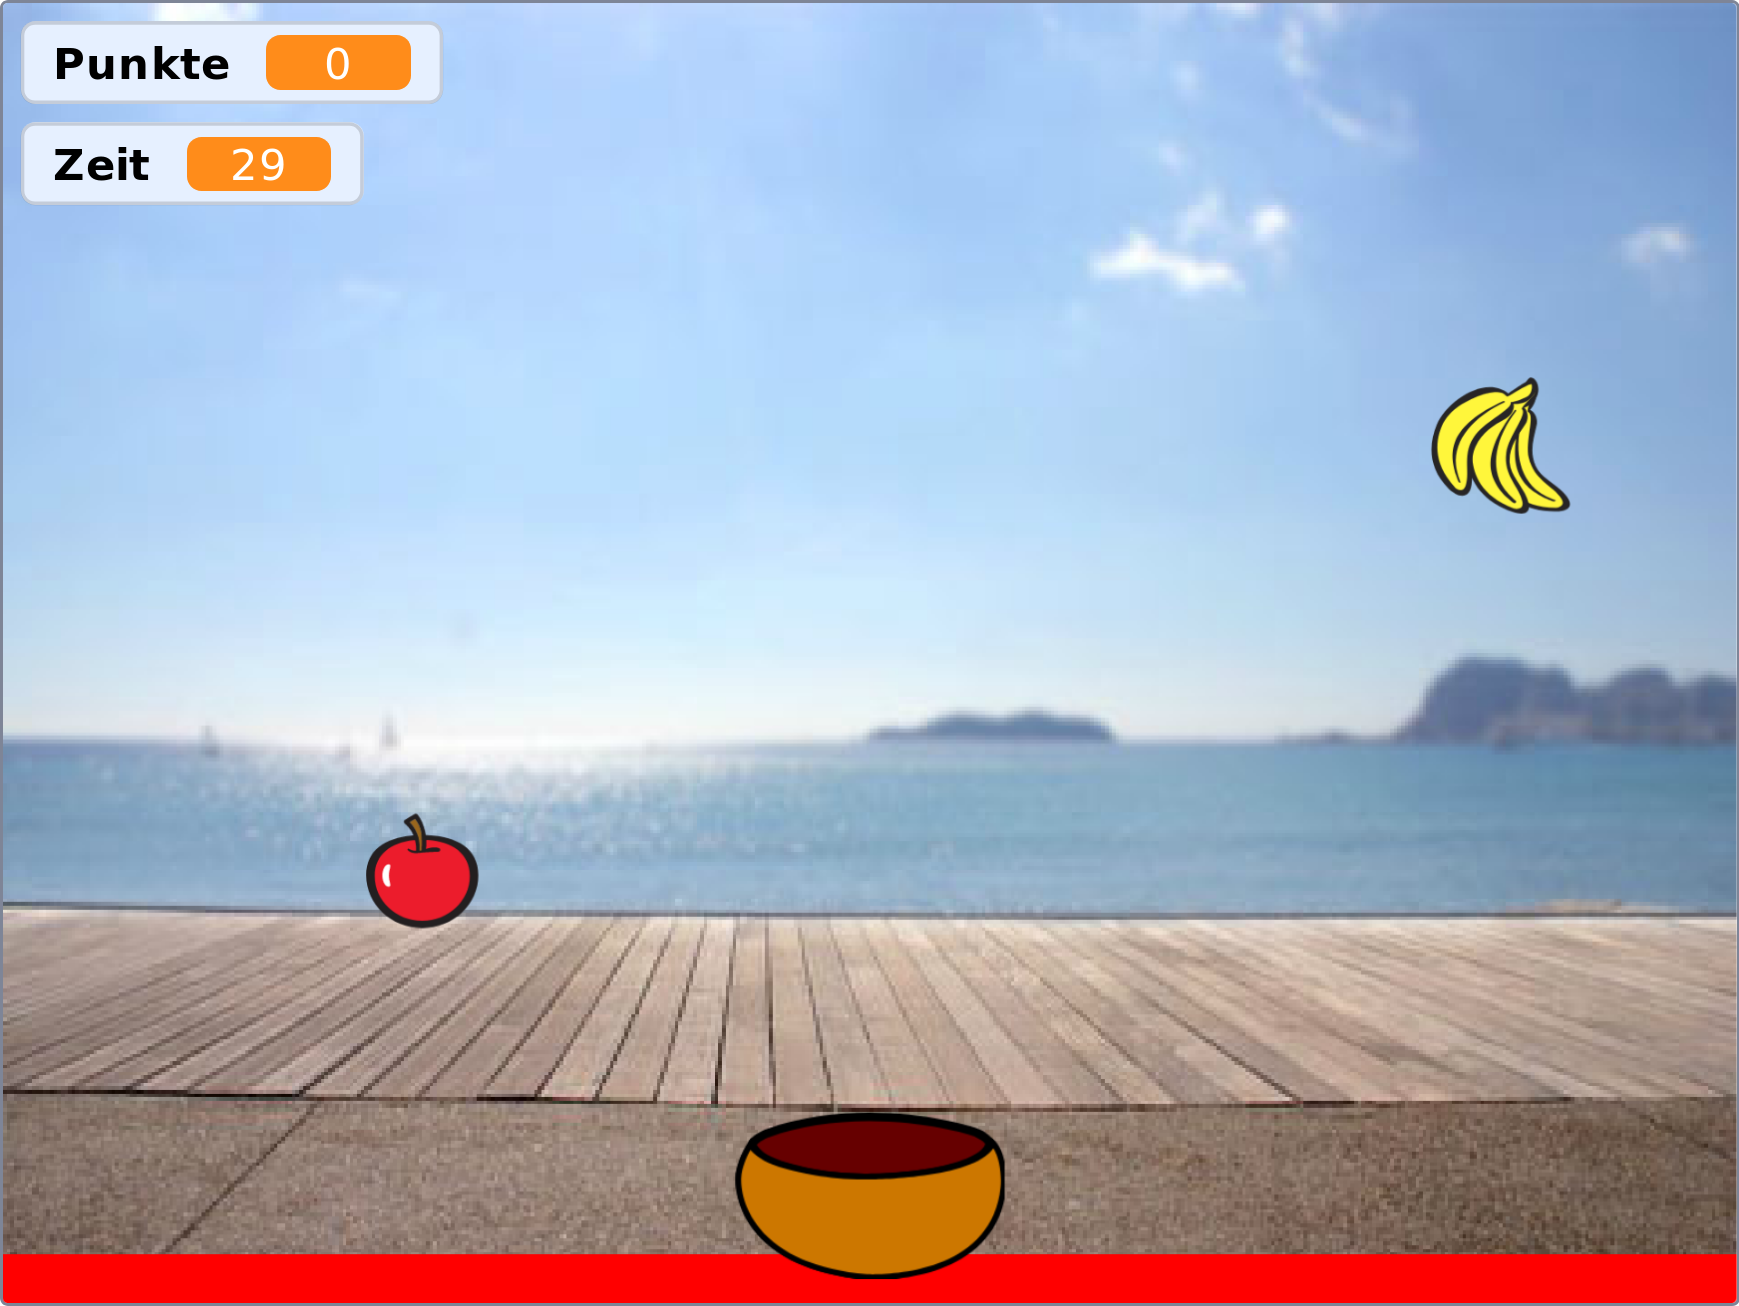
\includegraphics[height=.25\textheight]{scratch-stage}};

        \node[] at (0.0, 5.5) (inputtxt)  {\textbf{Input}};
        \node[] at (5.1, 5.5) (outputtxt) {\textbf{Output}};

        \draw [shorten >= 2pt, shorten <= 2pt, arrow] (input) -- (output);
    \end{tikzpicture}

    \bigskip

    \begin{tikzpicture}[scale=0.9, every node/.style={scale=0.9}]
        \node[box] at (-0.1, 4.0) (input) {
            \begin{minipage}{.28\textwidth}
                \begin{minted}[autogobble, breaklines, fontsize=\scriptsize, frame=none]{javascript}
                    t.inputImmediate({
                        device: 'mouse',
                        isDown: true,
                        x: 50,
                        y: 100
                    });
                \end{minted}
            \end{minipage}
        };

        \node[box] at (5.1, 4.0) (output) {
            \begin{minipage}{.28\textwidth}
                \begin{minted}[autogobble, breaklines, fontsize=\scriptsize, frame=none]{javascript}
                    sprite.x
                    sprite.y
                    sprite.rotation
                    sprite.sayText
                    sprite.costume
                    variable.value
                \end{minted}
            \end{minipage}
        };

        \node[] at (0.0, 5.5) (inputtxt)  {\textbf{Input}};
        \node[] at (5.1, 5.5) (outputtxt) {\textbf{Output}};

        \draw [shorten >= 2pt, shorten <= 2pt, arrow] (input) -- (output);
    \end{tikzpicture}

    \end{center}
\end{frame}

\begin{frame}\frametitle{How to test Scratch programs? Automating IO}
    \begin{figure}
        \centering
        \tikzset{>=latex,
                 arrow/.style={-{Latex[length=1.5mm, width=1.5mm]}},
                 label/.style={draw=none, text width=5.3cm, minimum height=0.5cm, text centered},
                   box/.style={draw,      text width=3.2cm, minimum height=0.7cm, text centered, rounded corners},
                     h/.style={fill=blue!10}}

        \begin{tikzpicture}
            \node[box, h] at ( 0.0, 3.0) (gui)           {Scratch GUI};
            \node[box]    at (-2.0, 1.5) (scratchvm)     {Scratch VM};
            \node[box]    at ( 2.2, 1.5) (scratchrender) {Scratch Renderer};
            \node[box, color=gray]   at (-2.0, 0.0) (program)       {Program};
            \node[box, color=gray]   at ( 2.2, 0.0) (htmlcanvas)    {HTML Canvas};

            \foreach \pp/\pf/\pt in {--/gui/scratchvm,
                                     --/gui/scratchrender,
                                     --/scratchvm/scratchrender,
                                     --/scratchvm/program,
                                     --/scratchrender/htmlcanvas}
            \draw[shorten >= 2pt, arrow] (\pf) \pp (\pt);
        \end{tikzpicture}

        \caption{General architecture of Scratch}
    \end{figure}
\end{frame}

\begin{frame}\frametitle{How to test Scratch programs? Automating IO}
    \begin{figure}[htpb]
        \centering
        \tikzset{>=latex,
                 arrow/.style={-{Latex[length=1.5mm, width=1.5mm]}},
                 label/.style={draw=none, text width=5.3cm, minimum height=0.5cm, text centered},
                   box/.style={draw,      text width=3.2cm, minimum height=0.7cm, text centered, rounded corners},
                     h/.style={fill=blue!10}}

        \begin{tikzpicture}
            \node[box]    at ( 0.00,  1.5) (testcode)      {Test Code};
            \node[box, h] at ( 0.00,  0.0) (whisker)       {Whisker};
            \node[box]    at (-2.00, -1.5) (scratchvm)     {Scratch VM};
            \node[box]    at ( 2.20, -1.5) (scratchrender) {Scratch Renderer};
            \node[box, color=gray]   at (-2.0, -3.0) (program)       {Program};
            \node[box, color=gray]   at ( 2.2, -3.0) (htmlcanvas)    {HTML Canvas};

            \foreach \pp/\pf/\pt in {--/testcode/whisker,
                                     --/whisker/scratchvm,
                                     --/whisker/scratchrender,
                                     --/scratchvm/scratchrender,
                                     --/scratchvm/program,
                                     --/scratchrender/htmlcanvas}
            \draw[shorten >= 2pt, arrow] (\pf) \pp (\pt);
        \end{tikzpicture}

        \caption{General architecture of Whisker}
    \end{figure}
\end{frame}

\begin{frame}[fragile]\frametitle{How to test Scratch programs? Automating IO}
    \tikzset{>=latex,
           arrow/.style={draw, -{Latex[length=1.5mm, width=1.5mm]}},
             put/.style={draw, minimum height=0.65cm, minimum width=1.75cm, rounded corners, fill=red!20, text width=2.4cm, text centered},
              vm/.style={draw, minimum height=1.75cm, minimum width=3.0cm, rounded corners, fill=white},
             gui/.style={draw, minimum height=2.6cm, minimum width=3.5cm, rounded corners, fill=blue!20},
         whisker/.style={draw, minimum height=2.6cm, minimum width=3.5cm, rounded corners, fill=green!20},
             box/.style={draw,text centered, rounded corners}}

    \hspace{2mm}\begin{tikzpicture}[scale=0.9, every node/.style={scale=0.9}]
        \node[box] at (0.0, 4.0) (input)  {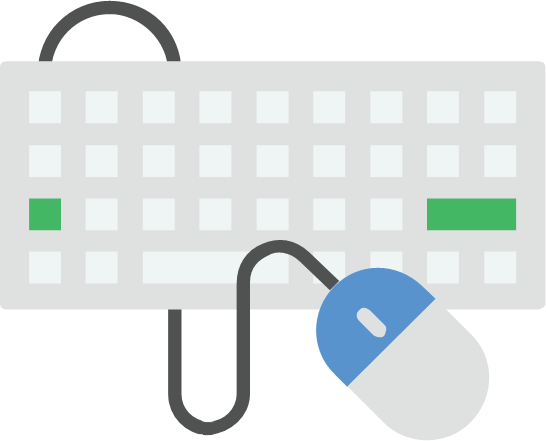
\includegraphics[height=.25\textheight]{mouse-keyboard}};
        \node[box] at (8.1, 4.0) (output) {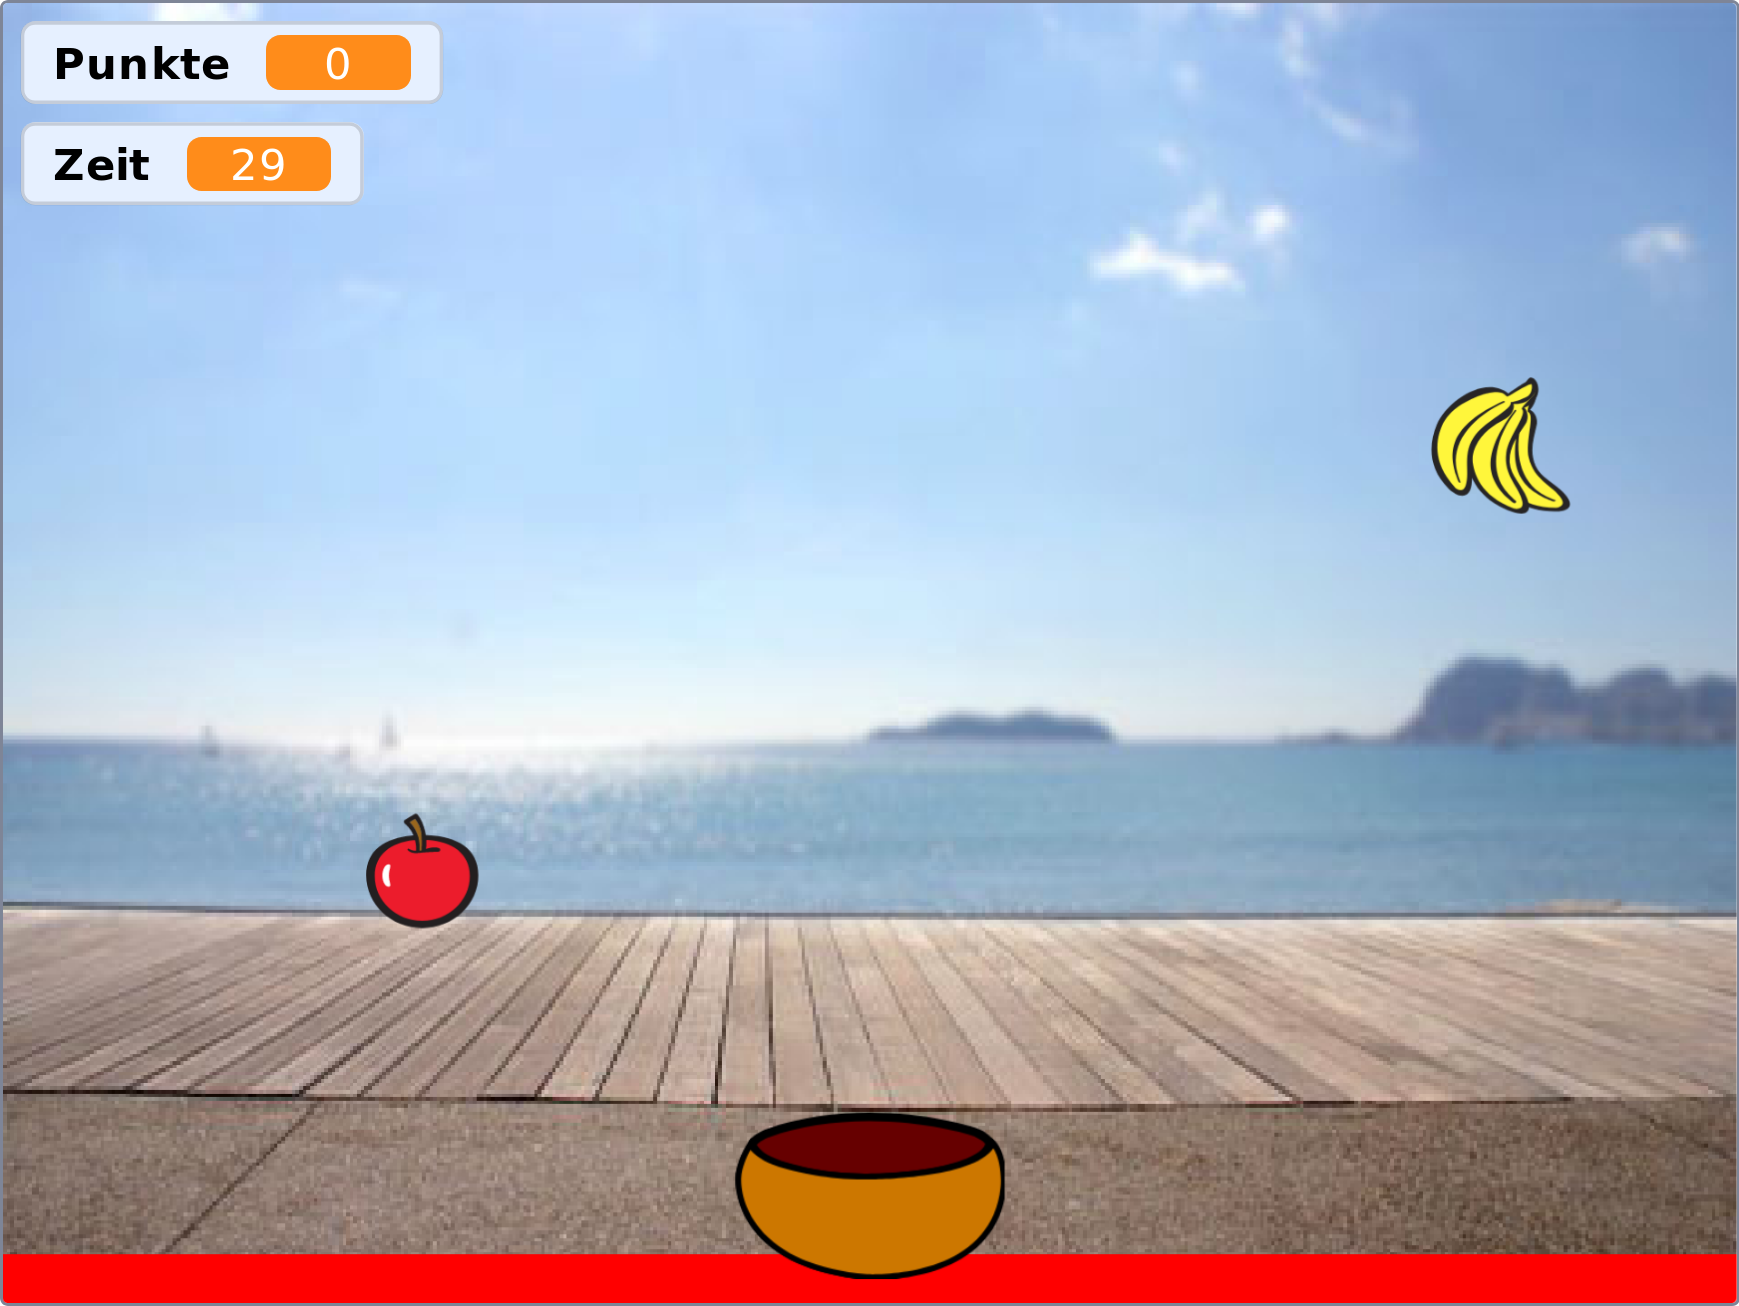
\includegraphics[height=.25\textheight]{scratch-stage}};

        \node[] at (0.0, 5.5) (inputtxt)  {\textbf{Input}};
        \node[] at (8.1, 5.5) (outputtxt) {\textbf{Output}};

        \begin{scope}[on background layer]
            \node[gui] at (4.0,  4.0)  (gui) {};
            \node[vm]  at (4.0,  3.75) (vm)  {};
        \end{scope}

        \node[put] at (4.0,  3.5) (put)     {\small Program under test};
        \node[]    at (4.0,  4.3) (vmtxt)   {\small Scratch VM};
        \node[]    at (4.0,  4.95) (guitxt) {\textbf{Scratch GUI}};

        \draw [shorten >= 2pt, shorten <= 2pt, arrow] (input) -- (gui);
        \draw [shorten >= 2pt, shorten <= 2pt, arrow] (gui)   -- (output);
    \end{tikzpicture}

    \bigskip

    \begin{tikzpicture}[scale=0.9, every node/.style={scale=0.9}]
        \node[box] at (-0.1, 4.0) (input) {
            \begin{minipage}{.28\textwidth}
                \begin{minted}[autogobble, breaklines, fontsize=\scriptsize, frame=none]{javascript}
                    t.inputImmediate({
                        device: 'mouse',
                        isDown: true,
                        x: 50,
                        y: 100
                    });
                \end{minted}
            \end{minipage}
        };

        \node[box] at (8.1, 4.0) (output) {
            \begin{minipage}{.28\textwidth}
                \begin{minted}[autogobble, breaklines, fontsize=\scriptsize, frame=none]{javascript}
                    sprite.x
                    sprite.y
                    sprite.rotation
                    sprite.sayText
                    sprite.costume
                    variable.value
                \end{minted}
            \end{minipage}
        };

        \node[] at (0.0, 5.4) (inputtxt)  {\textbf{Input}};
        \node[] at (8.1, 5.4) (outputtxt) {\textbf{Output}};

        \begin{scope}[on background layer]
            \node[whisker] at (4.0,  4.0)  (whisker) {};
            \node[vm]      at (4.0,  3.75) (vm)      {};
        \end{scope}

        \node[put] at (4.0,  3.5)  (put)        {\small Program under test};
        \node[]    at (4.0,  4.3)  (vmtxt)      {\small Scratch VM};
        \node[]    at (4.0,  4.95) (whiskertxt) {\textbf{Whisker}};

        \draw [shorten >= 2pt, shorten <= 2pt, arrow] (input)   -- (whisker);
        \draw [shorten >= 2pt, shorten <= 2pt, arrow] (whisker) -- (output);
    \end{tikzpicture}
\end{frame}

\begin{frame}
    \bigcenter{Whisker}
\end{frame}

\begin{frame}\frametitle{Whisker, Whisker's GUI}
    \begin{figure}
        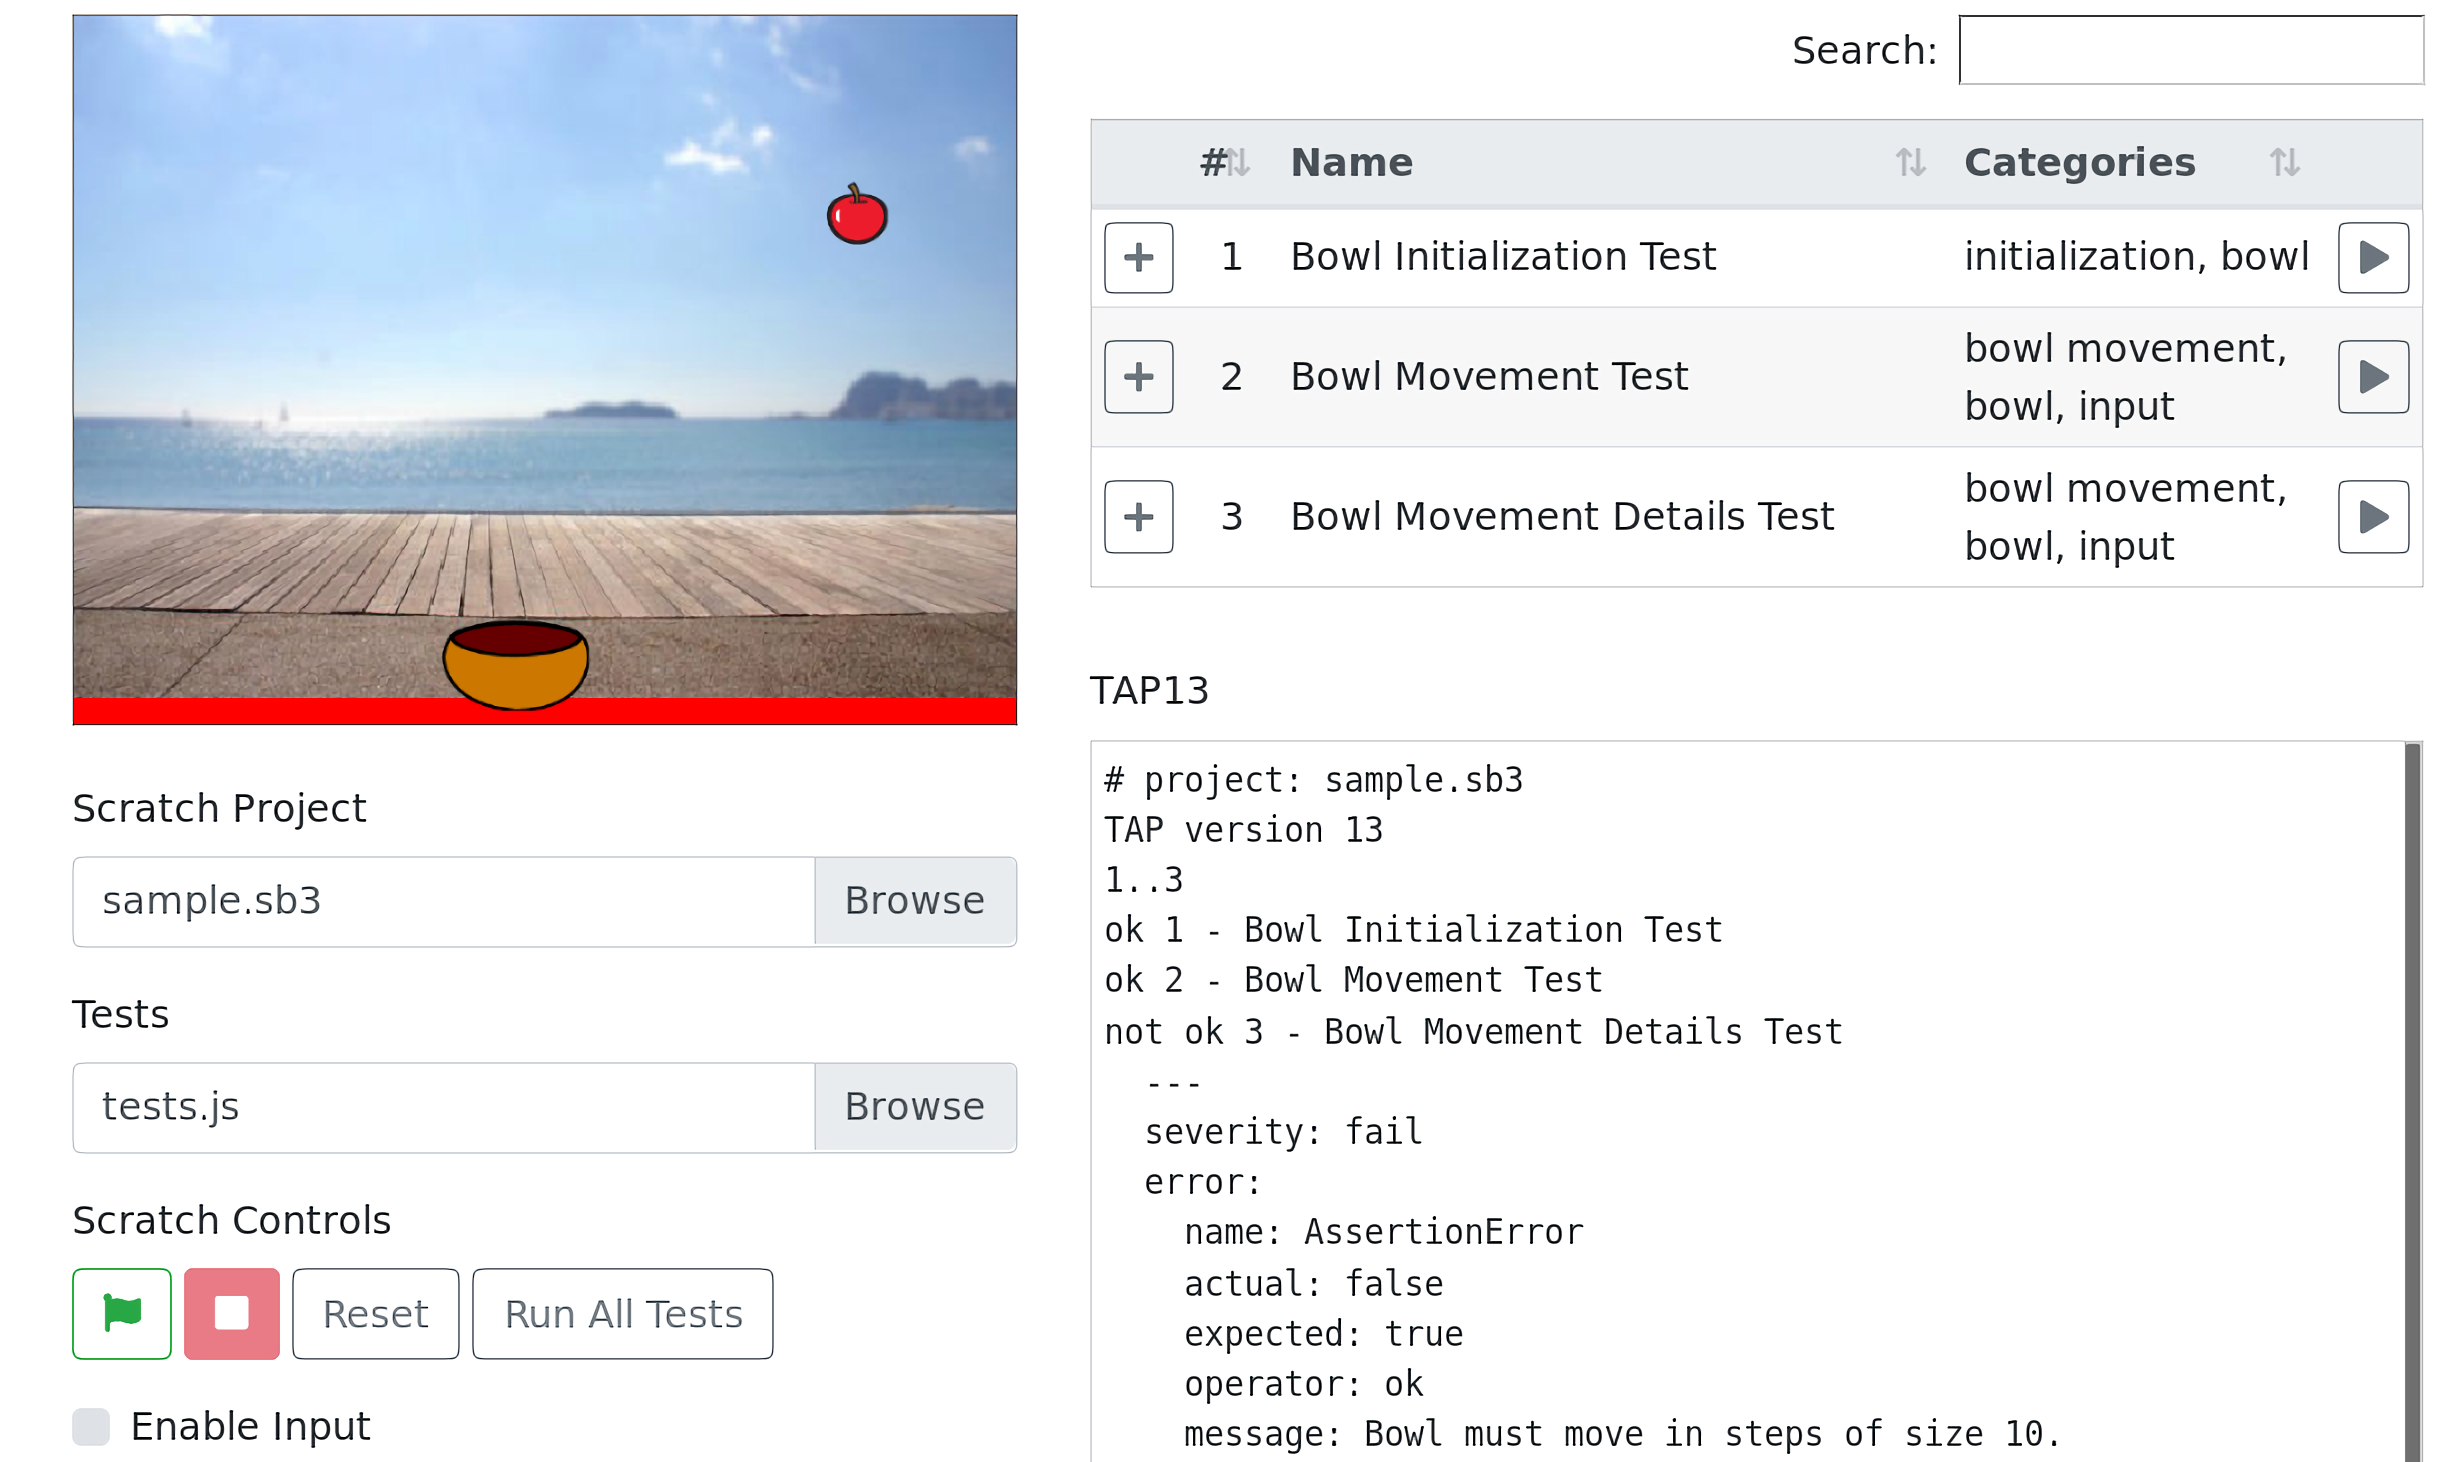
\includegraphics[width=\textwidth]{whisker-gui-big-upscaled}
        \caption{Whisker's GUI}
    \end{figure}
    % Whisker allows us to interact with the Scratch VM through a JavaScript API
\end{frame}

\begin{frame}[fragile]\frametitle{Whisker, Example Test}
    \vspace{-\bigskipamount}
    \begin{minipage}{.7\textwidth}\begin{tikzpicture}
        \node[opacity=1.0] (0,0) {
            \begin{minipage}{\textwidth}
                \begin{javascriptcode}
                    const test = async function (t) {
                        const sprite = t.getSprite('Sprite1');

                        await t.runForTime(100);
                        let oldX = sprite.x;

                        await t.runForTime(1000);

                        t.assert.ok(oldX === sprite.x);

                        t.inputImmediate({
                            device: 'keyboard',
                            key: 'right arrow',
                            isDown: true
                        });

                        await t.runForTime(1000);

                        t.assert.ok(oldX < sprite.x);
                    }
                \end{javascriptcode}
            \end{minipage}
        };
    \end{tikzpicture}\end{minipage}
\end{frame}

\begin{frame}[fragile]\frametitle{Whisker, Accessing Sprites and Variables}
    \vspace{-\bigskipamount}
    \begin{minipage}{.7\textwidth}\begin{tikzpicture}
        \node[opacity=0.35] (0,0) {
            \begin{minipage}{\textwidth}
                \begin{javascriptcode}
                    const test = async function (t) {
                        const sprite = t.getSprite('Sprite1');

                        await t.runForTime(100);
                        let oldX = sprite.x;

                        await t.runForTime(1000);

                        t.assert.ok(oldX === sprite.x);

                        t.inputImmediate({
                            device: 'keyboard',
                            key: 'right arrow',
                            isDown: true
                        });

                        await t.runForTime(1000);

                        t.assert.ok(oldX < sprite.x);
                    }
                \end{javascriptcode}
            \end{minipage}
        };
    \end{tikzpicture}\end{minipage}%
    \hspace{-.4\textwidth}%
    \begin{minipage}{.6\textwidth}
        \begin{javascriptcode}
            t.getSprite('Sprite1');
            t.getSprites(sprite => sprite.x > 100);
            t.getStage();

            sprite.getVariable('my variable');

            sprite.x;
            sprite.rotation;
            variable.value;

            sprite.old.x;
            sprite.old.rotation;
            variable.old.value;

            sprite.isTouchingEdge();
        \end{javascriptcode}
    \end{minipage}
\end{frame}

\begin{frame}[fragile]\frametitle{Whisker, Example Test}
    \vspace{-\bigskipamount}
    \begin{minipage}{.7\textwidth}\begin{tikzpicture}
        \node[opacity=1.0] (0,0) {
            \begin{minipage}{\textwidth}
                \begin{javascriptcode}
                    const test = async function (t) {
                        const sprite = t.getSprite('Sprite1');

                        await t.runForTime(100);
                        let oldX = sprite.x;

                        await t.runForTime(1000);

                        t.assert.ok(oldX === sprite.x);

                        t.inputImmediate({
                            device: 'keyboard',
                            key: 'right arrow',
                            isDown: true
                        });

                        await t.runForTime(1000);

                        t.assert.ok(oldX < sprite.x);
                    }
                \end{javascriptcode}
            \end{minipage}
        };
    \end{tikzpicture}\end{minipage}
\end{frame}

\begin{frame}[fragile]\frametitle{Whisker, Running the Program}
    \vspace{-\bigskipamount}
    \begin{minipage}{.7\textwidth}\begin{tikzpicture}
        \node[opacity=0.35] (0,0) {
            \begin{minipage}{\textwidth}
                \begin{javascriptcode}
                    const test = async function (t) {
                        const sprite = t.getSprite('Sprite1');

                        await t.runForTime(100);
                        let oldX = sprite.x;

                        await t.runForTime(1000);

                        t.assert.ok(oldX === sprite.x);

                        t.inputImmediate({
                            device: 'keyboard',
                            key: 'right arrow',
                            isDown: true
                        });

                        await t.runForTime(1000);

                        t.assert.ok(oldX < sprite.x);
                    }
                \end{javascriptcode}
            \end{minipage}
        };
    \end{tikzpicture}\end{minipage}%
    \hspace{-.4\textwidth}%
    \begin{minipage}{.6\textwidth}
        \begin{javascriptcode}
            await t.runForTime(1000);
            await t.runUntil(() => a > b, 1000);

            t.getRunTimeElapsed();
            t.getTotalTimeElapsed();

            t.greenFlag();
        \end{javascriptcode}
    \end{minipage}
\end{frame}

\begin{frame}[fragile]\frametitle{Whisker, Example Test}
    \vspace{-\bigskipamount}
    \begin{minipage}{.7\textwidth}\begin{tikzpicture}
        \node[opacity=1.0] (0,0) {
            \begin{minipage}{\textwidth}
                \begin{javascriptcode}
                    const test = async function (t) {
                        const sprite = t.getSprite('Sprite1');

                        await t.runForTime(100);
                        let oldX = sprite.x;

                        await t.runForTime(1000);

                        t.assert.ok(oldX === sprite.x);

                        t.inputImmediate({
                            device: 'keyboard',
                            key: 'right arrow',
                            isDown: true
                        });

                        await t.runForTime(1000);

                        t.assert.ok(oldX < sprite.x);
                    }
                \end{javascriptcode}
            \end{minipage}
        };
    \end{tikzpicture}\end{minipage}
\end{frame}

\begin{frame}[fragile]\frametitle{Whisker, Simulating Inputs}
    \vspace{-\bigskipamount}
    \begin{minipage}{.7\textwidth}\begin{tikzpicture}
        \node[opacity=0.35] (0,0) {
            \begin{minipage}{\textwidth}
                \begin{javascriptcode}
                    const test = async function (t) {
                        const sprite = t.getSprite('Sprite1');

                        await t.runForTime(100);
                        let oldX = sprite.x;

                        await t.runForTime(1000);

                        t.assert.ok(oldX === sprite.x);

                        t.inputImmediate({
                            device: 'keyboard',
                            key: 'right arrow',
                            isDown: true
                        });

                        await t.runForTime(1000);

                        t.assert.ok(oldX < sprite.x);
                    }
                \end{javascriptcode}
            \end{minipage}
        };
    \end{tikzpicture}\end{minipage}%
    \hspace{-.4\textwidth}%
    \begin{minipage}{.6\textwidth}
        \begin{javascriptcode}
            t.inputImmediate({
                device: 'keyboard',
                key: 'right arrow',
                isDown: true,
                duration: 100
            });
            t.addInput(1000, {
                device: 'mouse',
                x: 100, y: 200,
                isDown: true
            });
            t.addInput(2000, {
                device: 'text',
                text: 'some answer'
            });

            t.getMousePos();
            t.isKeyDown('space');
        \end{javascriptcode}
    \end{minipage}
\end{frame}

\begin{frame}[fragile]\frametitle{Whisker, Example Test}
    \vspace{-\bigskipamount}
    \begin{minipage}{.7\textwidth}\begin{tikzpicture}
        \node[opacity=1.0] (0,0) {
            \begin{minipage}{\textwidth}
                \begin{javascriptcode}
                    const test = async function (t) {
                        const sprite = t.getSprite('Sprite1');

                        await t.runForTime(100);
                        let oldX = sprite.x;

                        await t.runForTime(1000);

                        t.assert.ok(oldX === sprite.x);

                        t.inputImmediate({
                            device: 'keyboard',
                            key: 'right arrow',
                            isDown: true
                        });

                        await t.runForTime(1000);

                        t.assert.ok(oldX < sprite.x);
                    }
                \end{javascriptcode}
            \end{minipage}
        };
    \end{tikzpicture}\end{minipage}
\end{frame}

\begin{frame}[fragile]\frametitle{Whisker, Callbacks}
    \begin{itemize}
        \item Callbacks get executed every time a frame is rendered
        \item Make it possible to \textcolor{upfim}{track} and \textcolor{upfim}{react} to what the user sees
    \end{itemize}

    \begin{javascriptcode}
        t.addCallback(() => someList.push(sprite.x));

        const callback = t.addCallback(() => {
            if (sprite.visible) {
                t.inputImmediate({ device: 'mouse', isDown: true });
            } else {
                t.inputImmediate({ device: 'mouse', isDown: false });
            }
        });

        callback.disable();
        callback.enable();
        callback.isActive();
    \end{javascriptcode}
    % TODO: remove disable / enable / isActive
\end{frame}

\begin{frame}[fragile]\frametitle{Whisker, Constraints}
    \begin{itemize}
        \item Constraints \textcolor{upfim}{define conditions} that must hold for the program
        \item Like callbacks, constraints are checked (executed) every time a frame is rendered
    \end{itemize}

    \begin{javascriptcode}
        t.onConstraintFailure('fail');
        t.onConstraintFailure('nothing');

        const constraint = t.addConstraint(() => {
            t.assert.ok(sprite.visible === true,
                        'Sprite must always be visible.');
        });

        constraint.disable();
        constraint.enable();
        constraint.isActive();
    \end{javascriptcode}
    % TODO: remove disable / enable / isActive
\end{frame}

\begin{frame}[fragile]\frametitle{Whisker, Automated Input Generation}
    \begin{itemize}
        \item At a constant frequency, performs a random input from a pool
        \item Whisker can detect what inputs the program can react to
    \end{itemize}

    \begin{javascriptcode}
        t.setRandomInputInterval(150);

        t.registerRandomInputs([
          { device: 'keyboard', key: 'left arrow', duration: [50, 100] },
          { device: 'keyboard', key: 'right arrow', duration: [50, 100] },
          { device: 'mouse', x: [-100, 100], y: [-100, 100], weight: 0.5 }
        ]);

        t.detectRandomInputs({ duration: [50, 100] });
    \end{javascriptcode}
\end{frame}

\newcommand{\tablebox}[1]{
    \begin{tikzpicture}
         \node[draw, text width=7.5cm, minimum height=0.6cm, rounded corners] {\footnotesize #1};
    \end{tikzpicture}
}

\begin{frame}\frametitle{Whisker, Detecting Inputs}
    \scalebox{0.75}{
        \begin{tabular}{m{5.25cm}m{9.0cm}}
            \large Scratch Block(s) & \large Resulting Input(s) \\
            \vspace{3.5mm}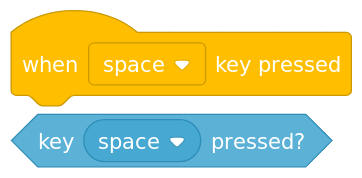
\includegraphics[scale=1.5]{scratch-input-blocks-1}\vspace{2mm} & \tablebox{(1) Press the respective keyboard key}                \\
            \vspace{3.5mm}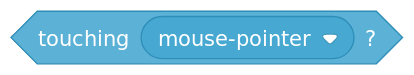
\includegraphics[scale=1.5]{scratch-input-blocks-4}\vspace{2mm} & \tablebox{(1) Move the cursor near / onto the respective sprite \\
                                                                                                      (2) Move the cursor to a random position}             \\
            \vspace{3.5mm}
\includegraphics[scale=1.5]{scratch-input-blocks-7}\vspace{2mm} & \tablebox{(1) Answer with a randomly generated string}          \\
            \vspace{3.5mm}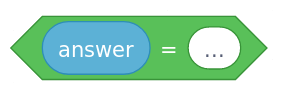
\includegraphics[scale=1.5]{scratch-input-blocks-8}\vspace{2mm} & \tablebox{(1) Answer with the compared string constant}         \\
            \huge ...                                                                     & \huge ...                                                       \\
        \end{tabular}
    }
\end{frame}
